\documentclass[border=5mm]{standalone}
\usepackage[utf8]{inputenc}
\usepackage[T1]{fontenc}
\usepackage{amsmath}
\usepackage{tikz}
\usepackage{pgfplots}
\pgfplotsset{compat=1.18}
\usetikzlibrary{arrows.meta}
\definecolor{utnblue}{RGB}{0, 51, 102}

% Ej6c: x(t)=tu(t), h(t)=cos(3t)u(t)
% y(t) = (1 - cos(3t))/9  u(t)
% Layout: fila superior x | h (escalas distintas), abajo y (ancho completo).

\begin{document}
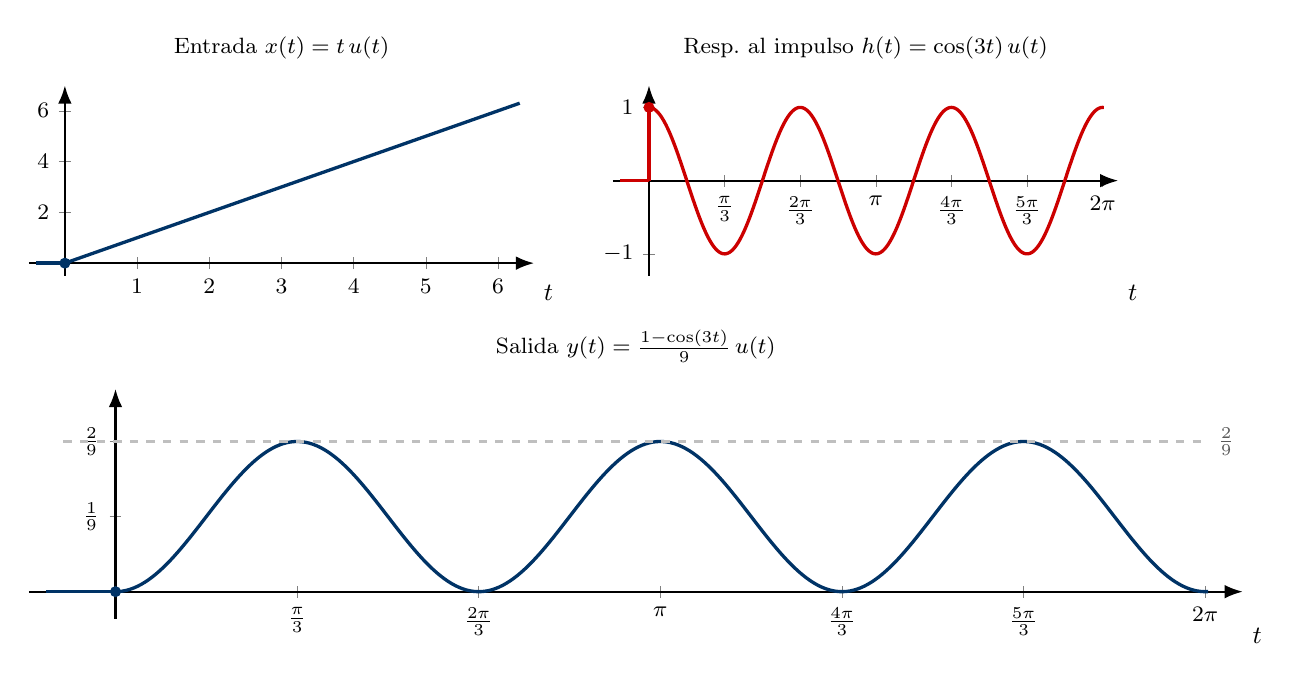
\begin{tikzpicture}[>=Latex, font=\small]

\colorlet{xcol}{utnblue}
\colorlet{hcol}{red!80!black}

% =====================================================================
% PANEL x(t) = t u(t)
% =====================================================================
\begin{axis}[
    name=panX,
    width=8cm, height=4cm,
    axis lines=center,
    xlabel={$t$},
    xlabel style={anchor=north west, at={(axis description cs:1,0)}},
    xmin=-0.5, xmax=6.5,
    ymin=-0.5, ymax=7,
    clip=false,
    axis line style={->, thick},
    xtick={0,1,2,3,4,5,6},
    ytick={0,2,4,6},
    every tick label/.style={font=\footnotesize},
    title={\footnotesize Entrada $x(t) = t\,u(t)$},
]
    \addplot[xcol, very thick, domain=-0.4:0, samples=2] {0};
    \addplot[xcol, very thick, domain=0:6.3, samples=2] {x};
    \fill[xcol] (axis cs:0,0) circle (2pt);
\end{axis}

% =====================================================================
% PANEL h(t) = cos(3t) u(t)
% =====================================================================
\begin{axis}[
    name=panH,
    at={(panX.east)}, anchor=west, xshift=1cm,
    width=8cm, height=4cm,
    axis lines=center,
    xlabel={$t$},
    xlabel style={anchor=north west, at={(axis description cs:1,0)}},
    xmin=-0.5, xmax=6.5,
    ymin=-1.3, ymax=1.3,
    clip=false,
    axis line style={->, thick},
    xtick={0, 1.047, 2.094, 3.14159, 4.189, 5.236, 6.283},
    xticklabels={$0$, $\tfrac{\pi}{3}$, $\tfrac{2\pi}{3}$, $\pi$, $\tfrac{4\pi}{3}$, $\tfrac{5\pi}{3}$, $2\pi$},
    ytick={-1, 0, 1},
    every tick label/.style={font=\footnotesize},
    title={\footnotesize Resp.\ al impulso $h(t) = \cos(3t)\,u(t)$},
]
    \addplot[hcol, very thick, domain=-0.4:0, samples=2] {0};
    \addplot[hcol, very thick, domain=0:6.3, samples=300]
        {cos(deg(3*x))};
    \draw[hcol, very thick] (axis cs:0,0) -- (axis cs:0,1);
    \fill[hcol] (axis cs:0,1) circle (2pt);
\end{axis}

% =====================================================================
% PANEL y(t) (ancho completo)
% =====================================================================
\begin{axis}[
    name=panY,
    at={(panX.below south west)}, anchor=north west, yshift=-1cm,
    width=17cm, height=4.5cm,
    axis lines=center,
    xlabel={$t$},
    xlabel style={anchor=north west, at={(axis description cs:1,0)}},
    xmin=-0.5, xmax=6.5,
    ymin=-0.04, ymax=0.3,
    clip=false,
    axis line style={->, thick},
    xtick={0, 1.047, 2.094, 3.14159, 4.189, 5.236, 6.283},
    xticklabels={$0$, $\tfrac{\pi}{3}$, $\tfrac{2\pi}{3}$, $\pi$, $\tfrac{4\pi}{3}$, $\tfrac{5\pi}{3}$, $2\pi$},
    ytick={0, 0.111, 0.222},
    yticklabels={$0$, $\tfrac{1}{9}$, $\tfrac{2}{9}$},
    every tick label/.style={font=\footnotesize},
    title={\footnotesize Salida $y(t) = \tfrac{1-\cos(3t)}{9}\,u(t)$},
]
    \addplot[utnblue, very thick, domain=-0.4:0, samples=2] {0};
    \addplot[utnblue, very thick, domain=0:6.3, samples=300]
        {(1-cos(deg(3*x)))/9};
    \fill[utnblue] (axis cs:0,0) circle (2pt);

    % asíntota superior 2/9
    \addplot[domain=-0.3:6.3, dashed, thick, gray!50] {2/9};
    \node[font=\footnotesize, gray!70!black, anchor=west]
        at (axis cs:6.3, 0.222) {$\tfrac{2}{9}$};
\end{axis}

\end{tikzpicture}
\end{document}
